\section{Introdução}

Os sistemas distribuídos representam uma das áreas mais importantes da computação moderna, sendo definidos como um conjunto de computadores independentes que se apresentam aos usuários como um sistema único e coerente \cite{tanenbaum2016sistemas}. Estes sistemas são caracterizados pela ausência de memória compartilhada, comunicação através de mensagens e pela independência de falhas entre os componentes \cite{coulouris2013sistemas}.

\begin{figure}[H]
\centering
\captionof{figure}{Arquitetura de Sistema Distribuído.}

\includegraphics[width=0.8\textwidth]{figure/placeholder.jpg}
\label{fig:arquitetura_distribuida}
{\fontsize{10pt}{\baselineskip}\selectfont
  Fonte: Adaptado de \citeonline{tanenbaum2016sistemas}}
\end{figure}

A evolução das redes de computadores possibilitou o desenvolvimento de sistemas distribuídos cada vez mais complexos e eficientes. Segundo \citeonline{kurose2021redes}, as redes modernas seguem uma abordagem em camadas que facilita a implementação e manutenção de protocolos de comunicação. O modelo TCP/IP, especificado inicialmente na RFC 793 \cite{rfc793:1981}, continua sendo a base fundamental para a comunicação em sistemas distribuídos.

Um dos principais desafios em sistemas distribuídos é o problema da sincronização e ordenação de eventos. \citeonline{lamport1978time} demonstrou que, na ausência de relógios perfeitamente sincronizados, é necessário estabelecer uma ordem lógica dos eventos através de algoritmos específicos. Este trabalho seminal estabeleceu as bases teóricas para muitos protocolos de consenso utilizados atualmente.

O teorema CAP, proposto por \citeonline{cap2000theorem}, estabelece que em sistemas distribuídos é impossível garantir simultaneamente consistência (Consistency), disponibilidade (Availability) e tolerância a partições (Partition tolerance). Este teorema fundamental influencia diretamente as decisões de projeto em sistemas distribuídos modernos.

Este relatório apresenta uma análise detalhada dos principais conceitos, algoritmos e tecnologias empregadas em redes e sistemas distribuídos, fundamentando-se em literatura acadêmica reconhecida e exemplos práticos de implementação.

\section{Fundamentos Teóricos e Metodologia}

\subsection{Algoritmos de Consenso Distribuído}

Os algoritmos de consenso são fundamentais para garantir a consistência em sistemas distribuídos. O algoritmo de Lamport para ordenação lógica de eventos é um dos pilares teóricos desta área.

\begin{algorithm}[H]
  \SetAlgoLined
  \KwData{Conjunto de processos $P = \{p_1, p_2, ..., p_n\}$}
  \KwIn{Evento local $e_i$ no processo $p_i$}
  \KwResult{Timestamp lógico ordenado}
  
  \Begin{
    Inicializar $LC_i = 0$ para cada processo $p_i$\;
    
    \For{cada evento local $e$ em $p_i$}{
      $LC_i = LC_i + 1$\;
      timestamp$(e) = LC_i$\;
    }
    
    \If{$p_i$ envia mensagem $m$ para $p_j$}{
      $LC_i = LC_i + 1$\;
      timestamp$(m) = LC_i$\;
      enviar $(m, LC_i)$ para $p_j$\;
    }
    
    \If{$p_j$ recebe mensagem $(m, LC_k)$ de $p_i$}{
      $LC_j = \max(LC_j, LC_k) + 1$\;
      processar mensagem $m$\;
    }
  }
  
  \caption{Algoritmo de Relógios Lógicos de Lamport}
  {\fontsize{10pt}{\baselineskip}\selectfont
    Fonte: Adaptado de \citeonline{lamport1978time}}
\end{algorithm}

\subsection{Protocolos de Comunicação em Redes}

A pilha de protocolos TCP/IP fornece a base para comunicação confiável em sistemas distribuídos. A Tabela~\ref{tab:protocolos} apresenta os principais protocolos utilizados em cada camada.

\begin{table}[H]
\centering
  \caption{Principais Protocolos da Pilha TCP/IP}
  \begin{tabular}{|l|l|l|l|}
      \hline
      \textbf{Camada} & \textbf{Protocolo} & \textbf{Função} & \textbf{RFC} \\
      \hline
      Aplicação & HTTP/HTTPS & Transferência de hipertexto & RFC 2616 \\
      \hline
      Aplicação & FTP & Transferência de arquivos & RFC 959 \\
      \hline
      Transporte & TCP & Transporte confiável & RFC 793 \\
      \hline
      Transporte & UDP & Transporte não confiável & RFC 768 \\
      \hline
      Internet & IP & Roteamento de pacotes & RFC 791 \\
      \hline
      Enlace & Ethernet & Acesso ao meio físico & IEEE 802.3 \\
      \hline
  \end{tabular}
  \label{tab:protocolos}
  \flushleft % Alinha à esquerda a referência

  {\fontsize{10pt}{\baselineskip}\selectfont
    Fonte: Adaptado de \citeonline{kurose2021redes}}
\end{table}


\section{Análise de Sistemas Distribuídos}

\subsection{Características e Propriedades}

Os sistemas distribuídos modernos devem atender a diversos requisitos não funcionais para garantir sua eficácia. As principais características incluem escalabilidade, disponibilidade, tolerância a falhas e transparência \cite{coulouris2013sistemas}.

A escalabilidade refere-se à capacidade do sistema de manter seu desempenho quando o número de usuários, recursos ou a carga de trabalho aumenta. Existem três tipos principais de escalabilidade: escalabilidade de tamanho, geográfica e administrativa \cite{tanenbaum2016sistemas}.

\subsection{Modelos de Arquitetura}

Os sistemas distribuídos podem seguir diferentes modelos arquiteturais, cada um com suas vantagens e desvantagens específicas:

\begin{enumerate}
    \item \textbf{Cliente-Servidor}: Modelo tradicional onde clientes fazem requisições a servidores
    \item \textbf{Peer-to-Peer (P2P)}: Todos os nós podem atuar como cliente e servidor
    \item \textbf{Arquitetura em Camadas}: Organização hierárquica de serviços
    \item \textbf{Microserviços}: Decomposição de aplicações em serviços pequenos e independentes
\end{enumerate}

\subsection{Implementação de Comunicação Distribuída}

O exemplo a seguir demonstra a implementação básica de um algoritmo de eleição em sistemas distribuídos:

\subsection{Algoritmo de Eleição em Anel}

Um exemplo prático de algoritmo distribuído é o algoritmo de eleição em anel, usado para eleger um coordenador em sistemas distribuídos.

\begin{algorithm}[H]
  \caption{Algoritmo de Eleição em Anel}
  \label{alg:eleicao_anel}
  \Entrada{Conjunto de processos $P = \{p_0, p_1, \ldots, p_{n-1}\}$ organizados em anel}
  \Saida{Eleição de um coordenador}
  
  \Inicio{
    \Comment{Quando um processo detecta falha do coordenador} \\
    \If{processo $p_i$ detecta falha do coordenador}{
      enviar mensagem ELEIÇÃO($p_i$) para próximo processo ativo no anel\;
      $participando \leftarrow verdadeiro$\;
    }
    
    \Comment{Ao receber mensagem de eleição} \\
    \If{$p_j$ recebe ELEIÇÃO($lista$)}{
      \If{$p_j \notin lista$}{
        adicionar $p_j$ à $lista$\;
        enviar ELEIÇÃO($lista$) para próximo processo no anel\;
        $participando \leftarrow verdadeiro$\;
      }
      \Else{
        \Comment{A mensagem deu volta completa no anel} \\
        $coordenador \leftarrow \max(lista)$\;
        enviar COORDENADOR($coordenador$) para próximo processo\;
      }
    }
    
    \Comment{Ao receber mensagem de coordenador} \\
    \If{$p_k$ recebe COORDENADOR($coord$)}{
      $coordenador \leftarrow coord$\;
      $participando \leftarrow falso$\;
      \If{$p_k \neq coord$}{
        enviar COORDENADOR($coord$) para próximo processo\;
      }
    }
  }

  \raggedright{\fontsize{10pt}{\baselineskip}\selectfont Fonte: Adaptado de \citeonline{tanenbaum2016sistemas}}
\end{algorithm}


\subsection{Análise de Desempenho}

A análise de desempenho em sistemas distribuídos envolve métricas como latência, throughput, disponibilidade e escalabilidade. A Figura~\ref{fig:comparacao_arquiteturas} apresenta uma comparação entre diferentes arquiteturas distribuídas.

\begin{figure}[H]
  \centering
  \caption{Comparação de Arquiteturas Distribuídas}
  \subfigure[Cliente-Servidor.\label{fig:cliente_servidor}]{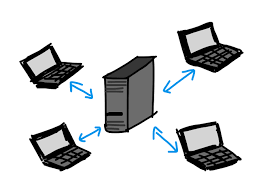
\includegraphics[scale=0.4]{figure/cliente-server.png}}
  \subfigure[Peer-to-Peer.\label{fig:p2p}]{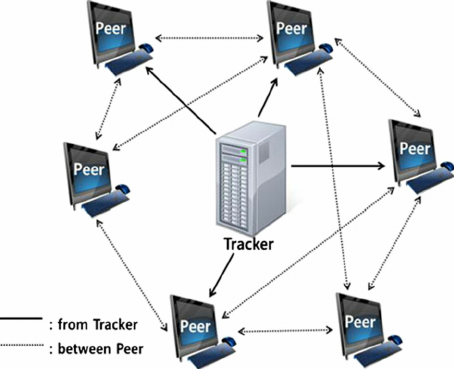
\includegraphics[scale=.4]{figure/peer-to-peer.png}}
  \label{fig:comparacao_arquiteturas}

  \raggedright{\fontsize{10pt}{\baselineskip}\selectfont Fonte: Adaptado de \citeonline{coulouris2013sistemas}}
\end{figure}

\subsection{Protocolos de Consenso}

Os protocolos de consenso são essenciais para manter a consistência em sistemas distribuídos. Algoritmos como Paxos, Raft e PBFT (Practical Byzantine Fault Tolerance) são amplamente utilizados em sistemas reais \cite{lamport1978time}. Cada protocolo apresenta diferentes garantias de segurança e vivacidade, adequadas para cenários específicos.



\section{Discussão e Considerações}

\subsection{Desafios Atuais}

Os sistemas distribuídos enfrentam diversos desafios que continuam sendo objeto de pesquisa ativa. Entre os principais desafios, destacam-se:

\begin{itemize}
    \item \textbf{Gerenciamento de Estado}: Manter consistência entre múltiplos nós
    \item \textbf{Detecção de Falhas}: Identificar e recuperar de falhas de rede e hardware
    \item \textbf{Partições de Rede}: Lidar com a separação temporária de nós
    \item \textbf{Escalabilidade}: Manter desempenho com crescimento do sistema
\end{itemize}

\subsection{Tendências Futuras}

As tendências emergentes em sistemas distribuídos incluem computação em borda (edge computing), blockchain, sistemas auto-adaptativos e inteligência artificial distribuída. Estas tecnologias promovem maior autonomia e eficiência dos sistemas \cite{coulouris2013sistemas}.

A evolução das redes 5G e 6G também impactará significativamente o design de sistemas distribuídos, possibilitando latências ultra-baixas e maior largura de banda \cite{cisco2019networking}.

\section{Conclusões}

Este trabalho apresentou uma análise abrangente dos fundamentos teóricos e práticos de redes e sistemas distribuídos. Os conceitos estudados demonstram a complexidade inerente à coordenação de múltiplos processos independentes e a importância de algoritmos bem fundamentados para garantir propriedades como consistência, disponibilidade e tolerância a falhas.

Os algoritmos de consenso, protocolos de comunicação e arquiteturas distribuídas estudados formam a base tecnológica para sistemas modernos como computação em nuvem, blockchain e Internet das Coisas (IoT). O teorema CAP e os trabalhos de Lamport sobre ordenação de eventos continuam sendo referências fundamentais para o desenvolvimento de novos sistemas.

As implementações práticas demonstraram que a escolha da arquitetura e dos algoritmos adequados depende das características específicas do domínio de aplicação. Sistemas que requerem alta disponibilidade podem optar por eventual consistency, enquanto sistemas bancários priorizam strong consistency.

Como trabalhos futuros, sugere-se a investigação de novos protocolos de consenso para ambientes com recursos limitados, como dispositivos IoT, e o desenvolvimento de frameworks que facilitem a implementação de sistemas distribuídos tolerantes a falhas bizantinas.

Os fundamentos apresentados neste relatório fornecem base sólida para compreensão e desenvolvimento de sistemas distribuídos eficientes e confiáveis, essenciais para a infraestrutura tecnológica moderna.
